w\chapter{Metodologia}

\section{Objetivos}

O objetivo deste capítulo é apresentar a metodologia utilizada para a
realização da pesquisa e contribuição tecnológica. A principal questão
a ser respondida é: como a visualização de software pode auxiliar na
interpretação das métricas coletas e calculadas por ferramentas de análise
de código?

Considerando esta questão, é importante ressaltar que existem incontáveis
destas ferramentas. Porém estas analisam apenas aspectos mui específicos
do software, e falham (algumas delas) em demostrar ao engenheiro de
qualidade a interpretação dos dados analisados \cite{deissenboeck2011}.

Neste trabalho serão unidas determinadas métricas, para gerar uma ou várias
visualizações que auxiliem o usuário do Mezuro a ter uma melhor interpretação do
resultado gerado por esta
ferramenta.

Como exemplo dessa união e para a construção do exemple de uso, é proposto
utilizar-se da decisão dos colegas Renan Costa Filgueiras e Vinícius Vieira
Meneses: foram escolhidas três métricas para a configuração da visualização em
radar: \textit{number of methods} (código: npm), \textit{number of public
methods} (código nom) e \textit{total number of modules} (código:
total\_modules); e a decisão de utilizar a biblioteca Javascript \textit{D3.js -
Data-Driven Documents} \cite{filgueiras2014mezuro}.

\section{Trabalhos Relacionados}

No artigo \textit{CodeCrawler – An Extensible and Language Independent 2D and
3D Software Visualization Tool}, \citeonline{lanza2005codecrawler}
desenvolveram uma ferramenta para visualização de software capaz de exibir
detalhes de uma forma polimétrica, que é capaz de mostrar informações como as
métricas do software, sua semântica e a relação entre as classes, por exemplo.
Segundo o autor essa visualização pode ser aplicada em vários contextos e não
somente em aspectos de software. Idealmente, a ferramenta é capaz de gerar
visualizações para software com grande número de linhas código. Porém é levado
em consideração a integração das visualizações em IDEs e essa solução não é
explorada. A utilização da técnica em diferentes ferramentas também não é
discutida.

Os autores, \citeonline{dosvisualizacc}, do \textit{Visualização de Software
Como Suporte ao Desenvolvimento Centrado em Métricas Orientadas a Objetivos}
criaram um plugin escrito em C++ para visualização de métricas OO, que são
coletadas pela ferramenta Qt Creator\footnote{\url{http://www.qt.io/ide/}}. As
métricas definidas foram: média de atributos por métodos em uma classe (MAC);
quantidade de métodos por classe (QMC); tamanho dos métodos por classe (TMC);
quantidade de atributos por classe (QAC); e quantidade de métodos públicos
(QMC). E nesse plugin os casos de uso ou funcionalidades no caso dessa
ferramenta são: calcular métricas: QAC; QMC; MAM; TMC; QMP. Além da
possibilidade de calcular a média das métricas, obter detalhes das métricas e
obter ajuda sobre as métricas. Um dos pontos importantes destacados no
resultado é a observação de que é possível garantir certo nível de qualidade
utilizando essas métricas até mesmo para projetos pequenos, com duas ou três
classes.

Porém a ferramenta só gera visualizações para aplicações escritas em C++, fator
limitante esse devido à incorporação do plugin à ferramenta Qt Creator. O
plugin calcula também apenas cinco métricas consideradas fundamentais para
avaliar a qualidade de um software. E o detalhamento de determinada classe e
uma visualização da evolução do projeto em uma linha do tempo também não foram
abordados neste trabalho.

O artigo dos autores \citeonline{ramosanalise}, cujo o título é Análise de
Métricas Estáticas para Sistemas JavaScripts, não trata necessariamente de
visualização de software, embora em várias figuras mostrem distribuições dos
projetos e seus respectivos valores das métricas escolhidas. Por tanto,
destacamos a escolha da ferramenta 
\textit{https://github.com/jared-stilwell/escomplex}\footnote{\url{https://github.com/jared-stilwell/escomplex}},
que analisa métricas de projetos escritos em JavaScript (linguagem que ainda
não é suportada para análise no Mezuro), e escolha das métricas que são: número
de módulos; linhas de código; número de parâmetros; complexidade ciclomática;
densidade de complexidade ciclomática; métricas de complexidade de Halstead; e
índice de manutenção.

É importante ressaltar também o artigo \textit{Understanding software evolution
using a combination of software visualization and software metrics}. Os
autores, \citeonline{ducasseunderstanding}, ressaltam que há uma grande
quantidade de dados hoje em circulação nos sistemas informatizados é este um
dos maiores problemas nas pesquisas de evolução de um software, e em alguns
casos as várias versões destes sistemas precisam ser analisadas em paralelo.
Então, considerando esta complexidade, uma técnica que pode auxiliar na
abordagem destas pesquisas é a visualização de software. É comentado sobre a
capacidade humana de observação de múltiplos aspectos de um problema em
paralelo e sua ligação direta com a visualização e o auxílio que possivelmente
esta trará o entendimento do sistema.

A técnica visual utilizada foi a matriz de evolução: combina visualização de
software com suas métricas \cite{lanza2001evolution}. Esta técnica permite
observar classes que merecem atenção, por exemplo por terem crescido ou
encolhido durante a vida útil do sistema. E a abordagem apresentada é
independente da linguagem, mesmo que em um dos estudos de caso tenha sido
analisado um software escrito em Smalltalk.

Dissertando um pouco mais sobre a técnica, \citeonline{ducasseunderstanding}
mostram suas minúcias. Cada coluna representa as diferentes versões do
software. Cada linha representa uma classe. E nessa técnica há algo importante
para este trabalho de conclusão de curso, onde é desejável trabalhar-se com o
software a evolução do mesmo durante certo tempo ou período.

Características que podem ser observadas na técnica:

\begin{itemize}
  \item Tamanho dos sistemas em termos de classes. Quanto mais linhas, maior o
  sistema;
  \item Classes adicionadas e removidas;
  \item Períodos decréscimo, estabilização ou crescimento do sistema durante a
  sua ``evolução''
  \item Classes \textit{Dayfly}. Classes com um tempo de vida pequeno, por
  exemplo que apenas apareceram em uma única versão do sistema;
  \item Classes que se mantêm (o contrário da característica observada no ponto
  anterior).
\end{itemize}

Porém, no artigo foi constato que essa representação não é precisa o suficiente.
A evolução então seria o uso das métricas de código-fonte.

A figura \ref{fig:evolutionMatrixAspects} foi extraída do artigo e mostra essas
características ou aspectos na evolução de um sistema, utilizando a técnica da
matriz de evolução. 

\begin{figure}[!htb]
  \centering
    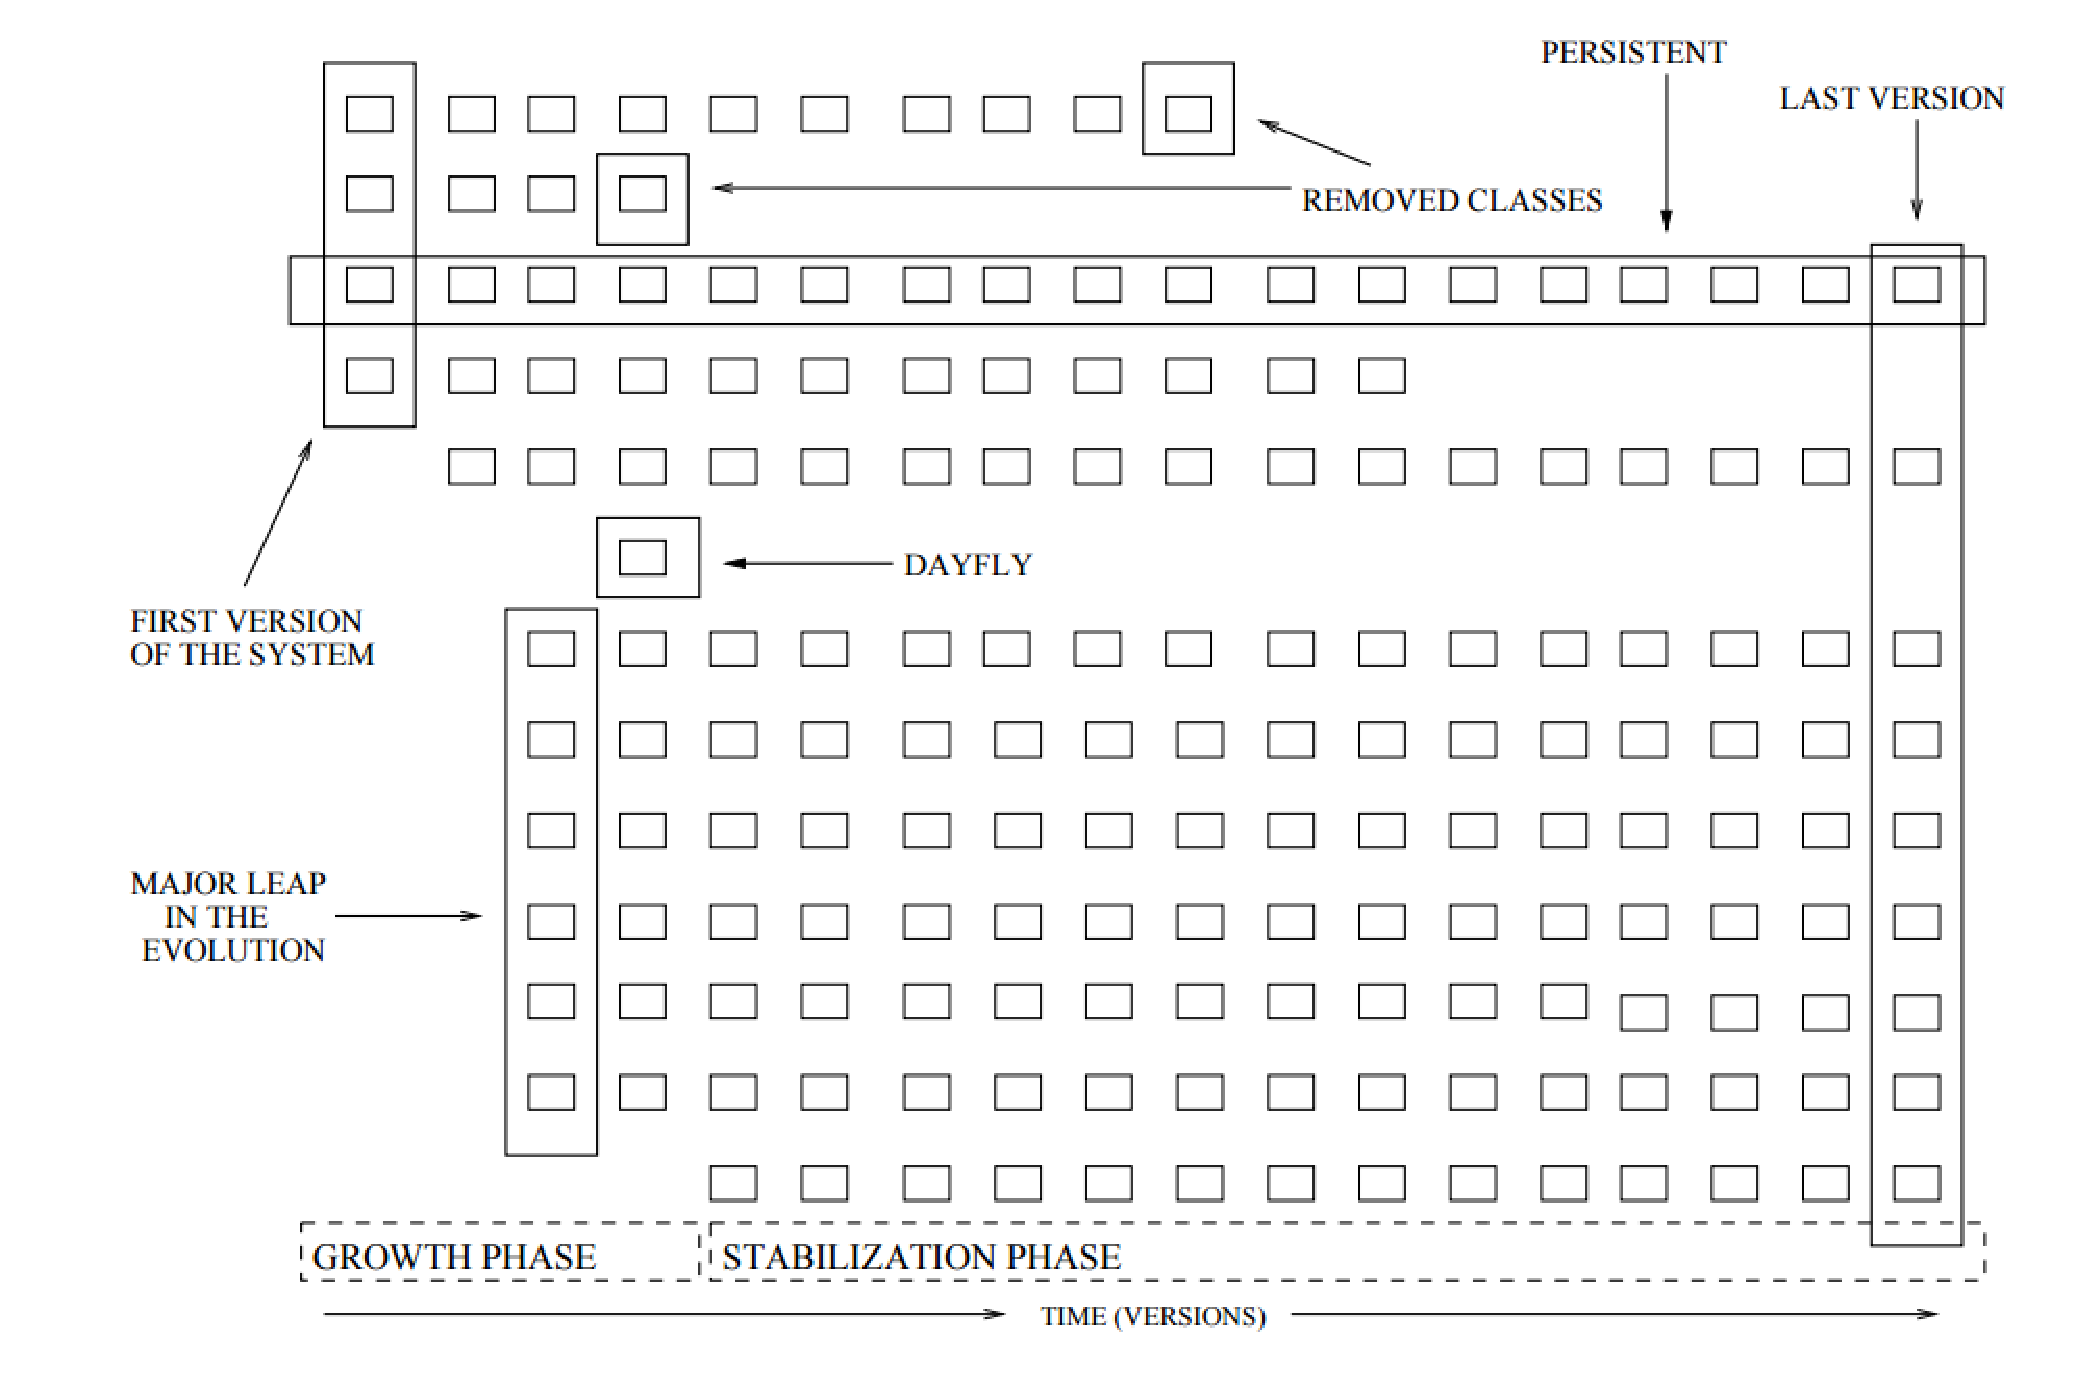
\includegraphics[keepaspectratio=true,scale=0.5]
    {figuras/evolutionMatrixAspects.eps}
  \caption{Aspectos da evolução de um sistema utilizando Matriz de Evolução
  \cite{ducasseunderstanding}}
  \label{fig:evolutionMatrixAspects}
\end{figure}


Ainda comentando sobre o artigo \textit{Understanding software evolution using
a combination of software visualization and software metrics}, destacamos o
como foi inserida esta evolução da utilização das métricas de código-fonte:
altura e a largura das caixas na visualização representam métricas das
classes. Métricas utilizadas: número de métodos (\textit{NOM}) e número de
atributos (\textit{NOA}).

E com as métricas definidas, foi feita uma categorização das classes em:

\begin{itemize}
  \item \textit{Pulsar}: uma classe que cresce de diminui durante o ciclo de
  vida do sistema;
  \item \textit{Supernova}: classe que de repente cresce bastante;
  \item \textit{White Dwarf}: classe que era grande, mas por algum motivo as
  suas responsabilidades foram dividas em outras classes e aquela diminui;
  \item \textit{Red Giant}: é uma classe considerada \textit{god class}
  \cite{riel1996object}, por muito tempo, ou seja: uma classe grande que
  implementa muitas funcionalidades;
  \item \textit{Idle}: classe constante, inativa, sem grandes modificações.
\end{itemize}

Concluindo, o artigo apresenta uma abordagem útil que talvez auxilie no
entendimento de um sistema. Porém é abordado no mesmo uma quantidade de
métricas pequena (embora significativa para o cotexto). Outro ponto negativo é
que em sistemas mui grandes, a visualização pode esbarrar em limitações de
exibição em uma única tela. E a abordagem pode apresentar problemas com nomes
repetidos de classes (considerando que este pode ser ou não um erro no
desenvolvimento de um sistema).

\section{Questão Problema e Hipóteses}

Reforçando a questão problema (QP), foram levantadas estas outras abaixo:

\begin{itemize}
  \item QP1 - Como a visualização de software pode auxiliar na
  interpretação das métricas coletadas e calculadas pelo Mezuro?
  \item QP2 - Quais técnicas de visualização que melhor se adequam ao
  contexto do Mezuro, possibilitando a aplicação em qualquer contexto de
  configuração?
  \item QP3 - Como representar as diferentes perspectivas sobre o processo
  de desenvolvimento e o produto de software?
\end{itemize}

As hipóteses são:

\begin{itemize}
  \item H1 - Não haverá uma visualização única para todas as métricas.
  \item H2 - Algumas métricas poderão ser apresentadas de uma forma combinada
  em uma única representação/visualização.
\end{itemize}

% TODO: elaborar e documentar as hipóteses

\section{O Mezuro}

O projeto Mezuro é uma ferramenta para extração, análise e interpretação de
métricas de código-fonte. De uma forma geral, ele é dividido em duas partes:
para o processamento e para o cálculo é utilizado o Kalibro, que é um
\textit{webservice}; e o Prezento para a interface gráfica (uma aplicação
\textit{Web}) \cite{meirellesCibse2015}. Sob a licença
\textit{Affero General Public License version 3} (AGPLv3), o Mezuro permite que
o usuário crie, salve e edite ``configurações'' que são um conjunto de
métricas escolhidas por este e um ``grupo de leitura'' para provimento de uma
interface gráfica de um conjunto de leitura que tenha algum sentido quando
agrupadas, por exemplo: com a pontuação x, a métrica terá o ``rótulo'' ``BOM'' e
será atribuído à ela a cor amarela; com a pontuação x + 2, a métrica terá o
``rótulo'' ``ÓTIMO'' e estará com a cor verde. As cores são para destacar a
interpretação e são definidas com valores hexadecimal \cite{camarinhaOSS2015}.

O Kalibro, citado no parágrafo anterior, foi inicialmente escrito em Java para
compor uma das ferramentas do projeto QualiPSo (\textit{Quality Platform for
Open Source Software}). Já possuía maioria das funcionalidades presentes na
versão atual do Mezuro. Uma delas, bastante prática, é a de fornecer apenas o
URL do código compactado em arquivo ZIP ou TARBALL, ou o link para as
aplicações de controle de versão em SVN ou GIT, mais a escolha de uma
configuração, para iniciar a análise \cite{camarinhaOSS2015}. Em 2013 o Mezuro
passou a ser reescrito em Ruby, com objetivo de manter na mesma tecnologia as
camadas da arquitetura. Mudança justificada também pela necessidade do
processamento dos cálculos e da análise. A carga de requisições, mais a
quantidade de núcleos que o servidor possuía, faziam com que a versão original
do Kalibro ficasse debilitado em seu fluxo de execuções. Outra vantagem dessa
reescrita é a facilidade com que novos contribuidores puderam/poderão entender
todo o funcionamento dessa parte do Mezuro. Algumas funcionalidades foram
eliminadas por serem consideradas não essenciais. E grande parte da primeira
versão do Kalibro está presente na gema
kalibro\_gem\footnote{\url{https://rubygems.org/gems/kalibro_gem}}
\cite{meirellesCibse2015}.

% TODO: a gem kalibro\_gem e a kalibro\_client são a mesma coisa? A kalibro\_gem
% foi descontinuada?)

% Sobre o Prezento

O Kalibro foi construído, nos primórdios, como um plugin da rede social
Noosfero. Com a decisão de reescrevê-lo em Ruby, a antiga interface gráfica,
que era aproveitada do Noosfero, foi também reescrita nesta
tecnologia. O Prezento, desenvolvido utilizando o \textit{framework} para
desenvolvimento de aplicações \textit{Web}
Ruby on Rails\footnote{\url{http://guides.rubyonrails.org/getting_started.html}},
é a redesenha e atual interface.

% Sobre a arquitetura do Mezuro

% (Eu preciso falar do QualiPSo?  Não!)

O projeto QualiPSo, iniciado em meados de 2007, tinha como objetivo aprimorar
as práticas de desenvolvimento aberto à época para atingir o reconhecimento e
confiabilidade que o FOSS possui hoje \cite{messias2012}.

\subsection{Arquitetura e principais funcionalidades do Mezuro}

Com a reescrita, a arquitetura do Mezuro foi dividida em três serviços:

\begin{itemize}
  \item Prezento: para a interface gráfica do usuário
  \item Kalibro Processor: para a análise do código
  \item Kalibro Configurations: para o gerenciamento das configurações
\end{itemize}

A decisão de dividir o Kalibro em serviços separados foi tomada para deixar
cada um deles com menos responsabilidades, facilitando a manutenção e evolução
\cite{camarinhaOSS2015}. E a comunicação entre estes serviços é feita através
do Kalibro Client: um quarto software também escrito em Ruby, mantendo a
escolha de centralização em uma única tecnologia. E para simplificar a
implementação, também foi decidido que a comunicação entre os serviços seria
RESTful.

As figuras a seguir demonstram como a comunicação funciona, um diagrama UML de
sequência do processo de criação de uma configuração chegando ao estágio em que
são expostos os resultados finais de uma análise após a reescrita da interface
gráfica, e outra que demonstra o estado atual do projeto.

\begin{figure}[!htb]
	\centering
    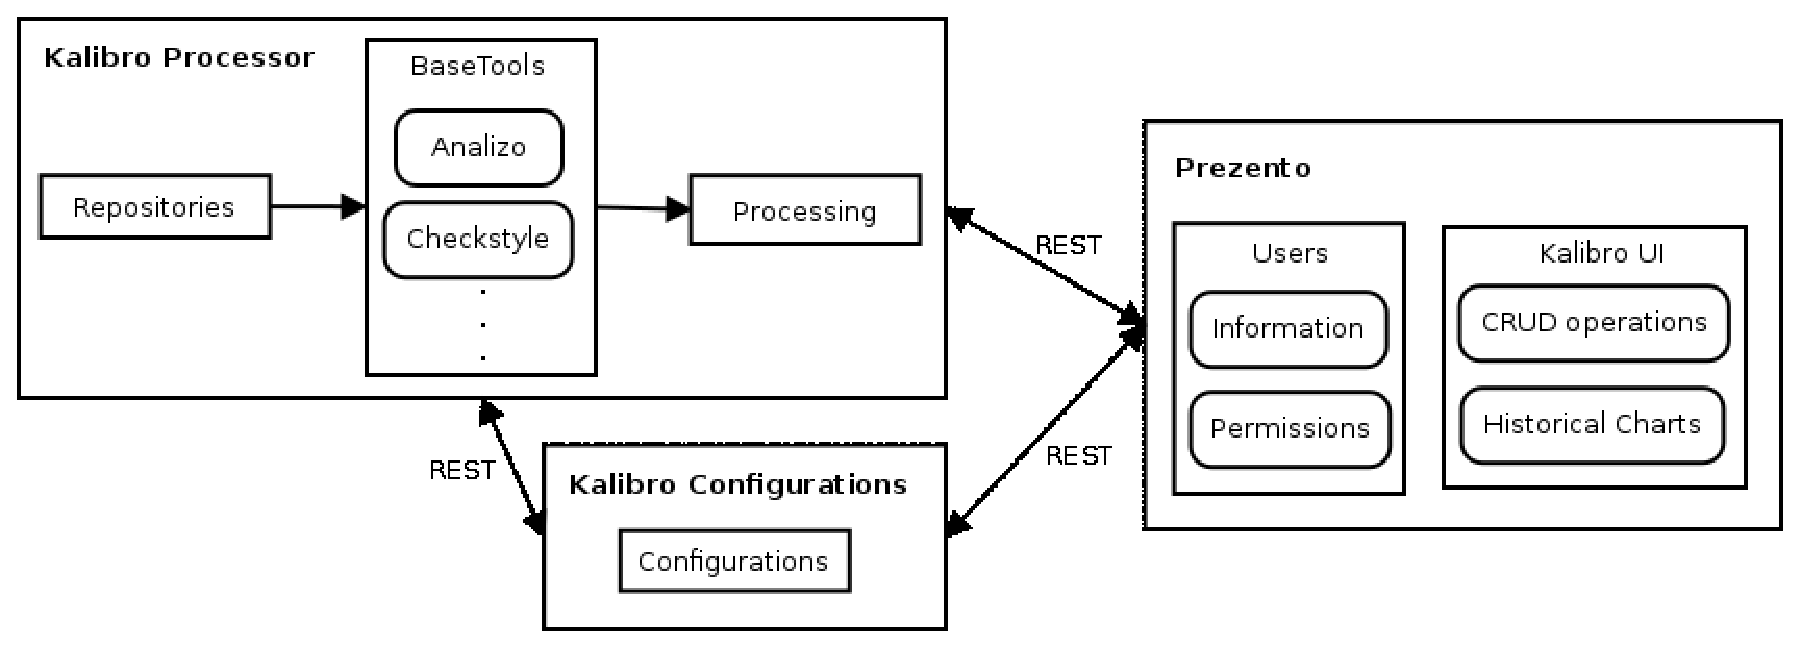
\includegraphics[keepaspectratio=true,scale=0.5]
    {figuras/mezuroCloudArch.eps}
  \caption{Arquitetura do Mezuro \cite{camarinhaOSS2015}}
	\label{fig:mezuroNoosferoArch}
\end{figure}

\begin{figure}[!htb]
	\centering
    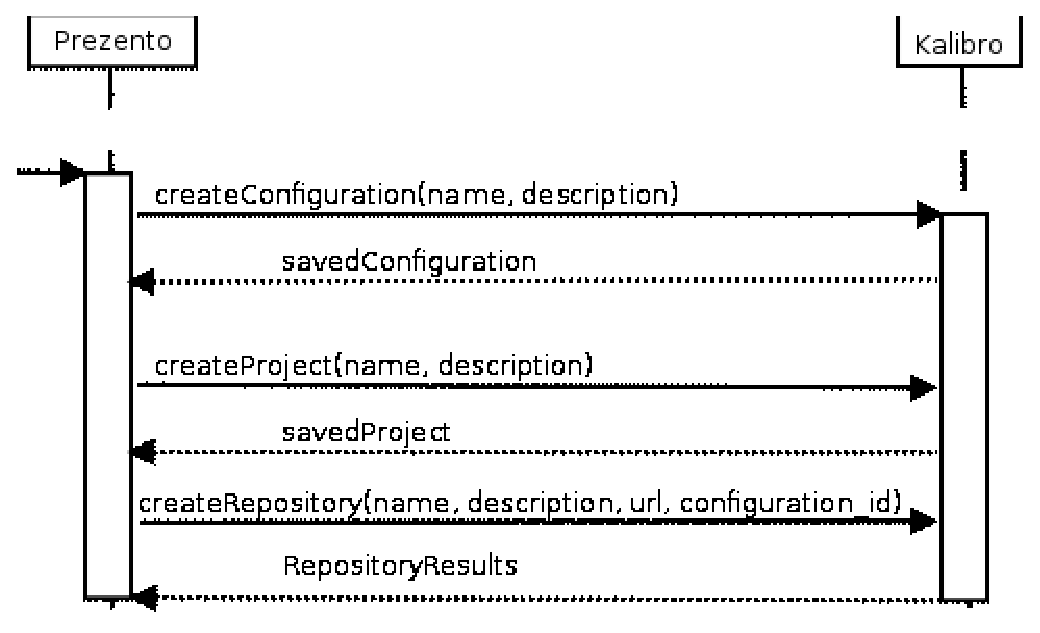
\includegraphics[keepaspectratio=true,scale=0.7]
    {figuras/prevProcessingSeqDiag.eps}
  \caption{Arquitetura do sistema ao fim da reescrita da interface gráfica
  \cite{meirellesCibse2015}}
	\label{fig:prevProcessingSeqDiag}
\end{figure}

\begin{figure}[!htb]
	\centering
    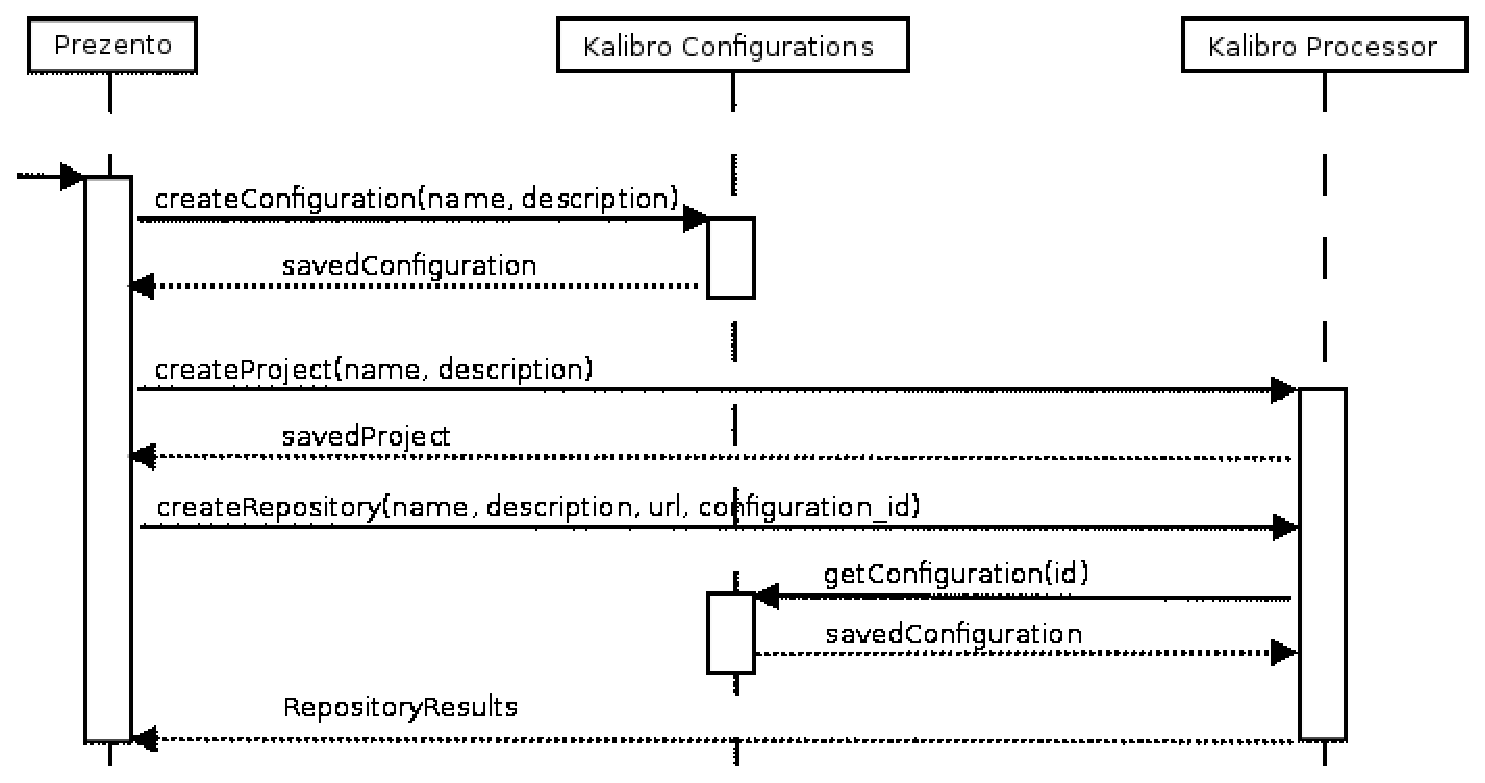
\includegraphics[keepaspectratio=true,scale=0.5]
    {figuras/processingSeqDiag.eps}
  \caption{Arquitetura do sistema ao fim da reestruturação do Kalibro
  \cite{meirellesCibse2015}}
	\label{fig:processingSeqDiag}
\end{figure}

\newpage

Segundo \citeonline{camarinhaOSS2015}, as principais ``funcionalidades podem ser
divididas em dois grupos:

\begin{itemize}
  \item Projeto
    \begin{itemize}
    \item \textit{Download} do código-fonte a partir de repositórios (Git,
    Subversion, Bazaar etc) ou via arquivo compactado;
        \item Escolha da periodicidade do processamento do código (1 dia, 2 dias,
        semanal, quinzenal e mensal);
        \item Escolha de qual configuração de métricas cada repositório irá
        utilizar;
        \item Nota de cada métrica da configuração para cada arquivo do
        repositório;
        \item Análise gráfica de cada arquivo do repositório por meio de um
        gráfico de pontos com notas ao longo do tempo;
        \item Resultados públicos e acessíveis à comunidade.
    \end{itemize}
    \item Configuração
    \begin{itemize}
    \item Criação de configuração e a possibilidade de clonagem;
        \item Estatísticas sobre as configurações mais populares dentro da
        comunidade;
        \item Criação de intervalos qualitativos associados aos valores das
        métricas;
        \item Criação de grupos de leitura para a interpretação textual dos
        resultados das métricas;
        \item Combinações de métricas nativas para criação de análises compostas
        e mais complexas.''
    \end{itemize}
\end{itemize}
''
TODO: consertar estas aspas na citação direta

\newpage

\section{A Decisão de utilizar o Mezuro}

Para este trabalho de conclusão de curso a ferramenta de de análise de código
fonte escolhida foi o Mezuro pois: o aluno já participou da evolução de parte
de algumas funcionalidades; a ferramenta proporciona ao usuário a análise
periódica do projeto, o que atende ao desejado como contribuição tecnológica
das visualizações geradas serem demonstradas ao longo do tempo; por ser uma
plataforma livre; fácil contato com os mantenedores; e por esta plataforma
sempre utilizar as últimas versões estáveis do Ruby e do Rails, ou seja,
por utilizar o que há de mais atual nestas tecnologias.

É importante ressaltar que outras ferramentas de análise de código poderão ser
utilizadas para geração da visualização proposta neste trabalho. Pois o fluxo
básico de execução permitirá tal geração, a saber: análise pela ferramenta,
dados exportados de forma determinada para anteder a leitura da biblioteca JS,
geração da visualização em um terceiro serviço local ou remoto.

E o ideal é que este trabalho sirva como base para a criação de futuras
visualizações para o Mezuro em si.

O foco do desenvolvimento, por tanto, será na camada de \textit{GUI} do Mezuro,
chamada Prezento.

\section{Proposta de Evolução da Visualização}

A atividade de contribuição tecnológica tem como objetivo selecionar métricas
com um certo nível  de similaridade e importância quando unidas, e a exibição de
tais por meio de uma das técnicas de visualização estudadas. Esta exibição
poderá ser uma nova página ou passo dentro do fluxo percorrido pelo usuário ao
utilizar o Mezuro para o monitoramento do código, ou ainda estar contida nas
informações gerais dos repositórios registrados na plataforma.

As etapas para que serão seguidas para elaboração desta atividade estão descrita
nos itens abaixo e a figura \ref{fig:metodotologia_atividades} ilustra e
encadeamento destas etapas:

\begin{figure}[h]
  \centering
    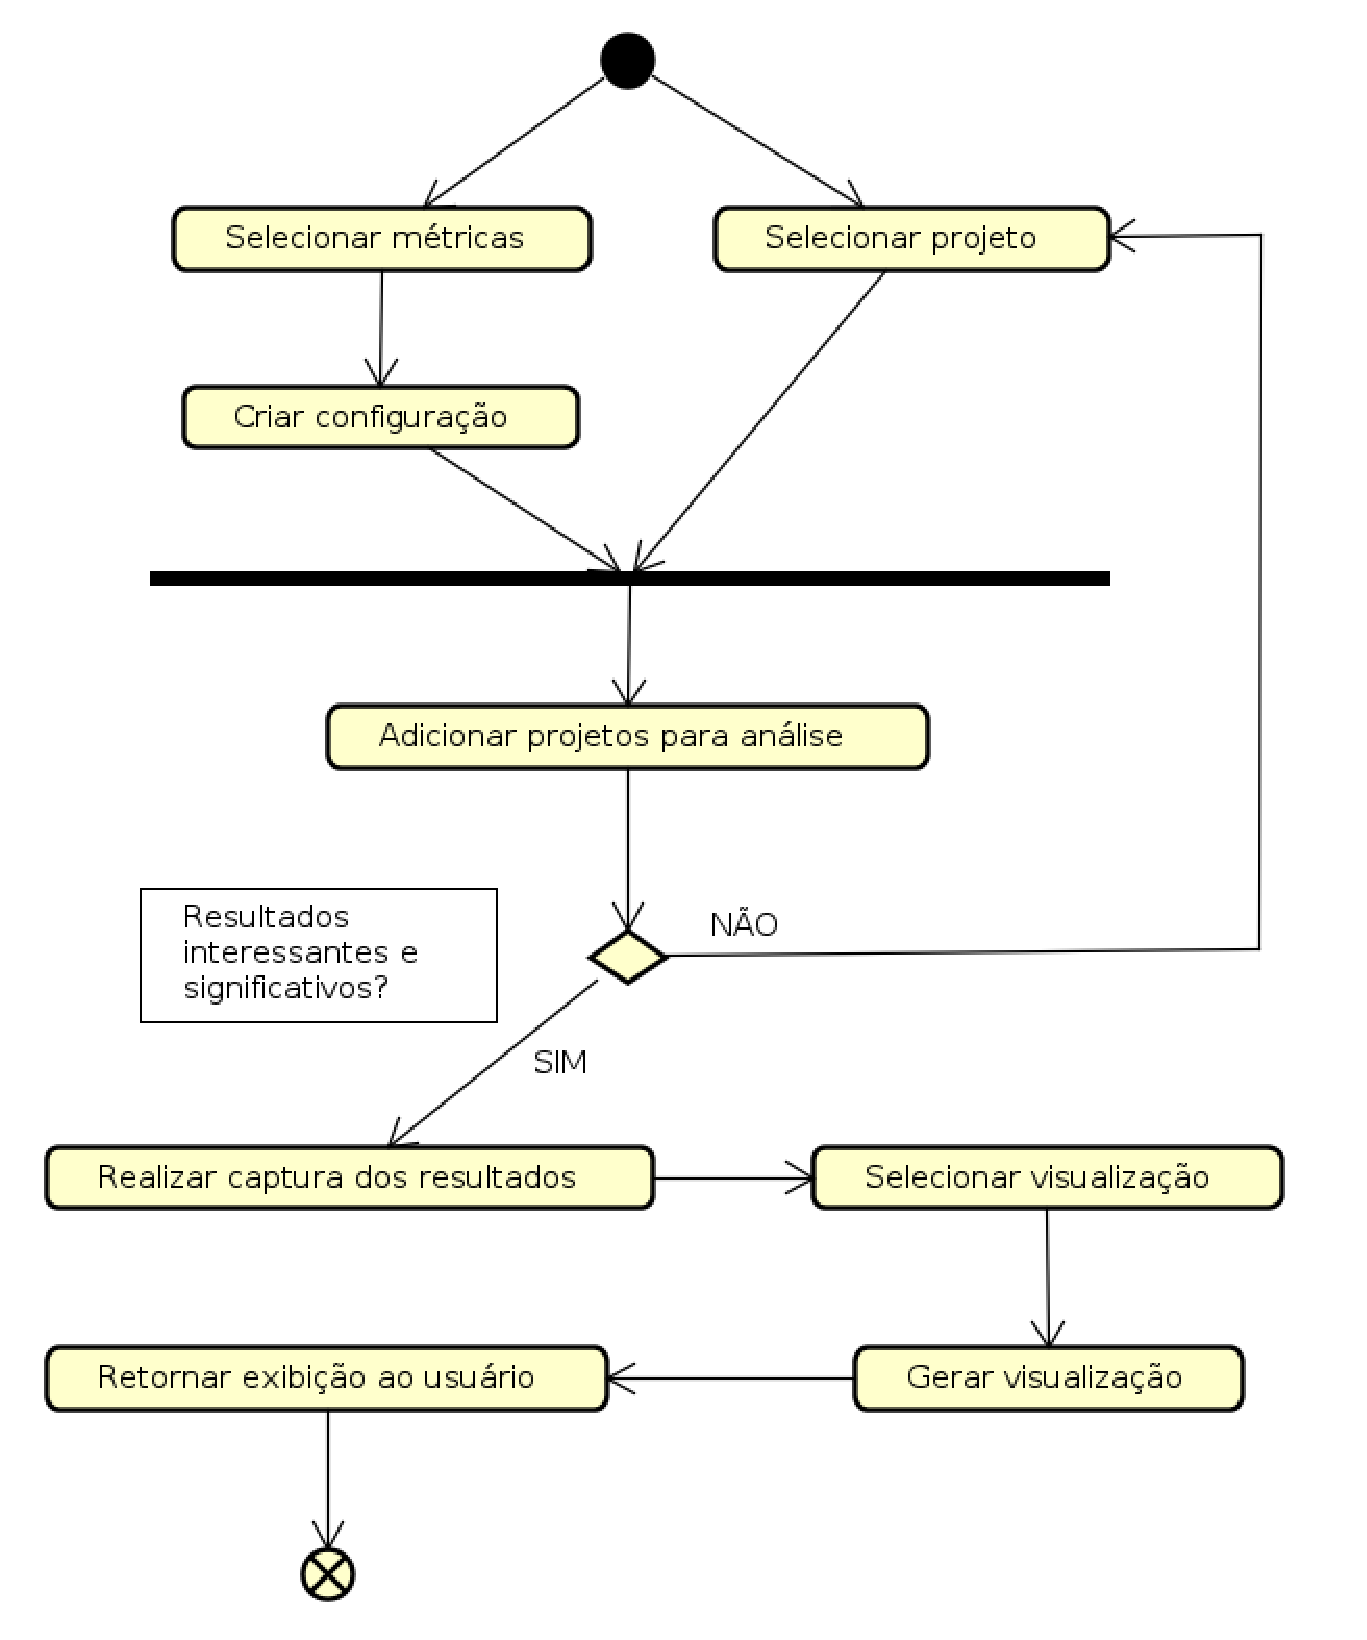
\includegraphics[keepaspectratio=true,scale=0.5]
    {figuras/metodotologia_atividades.eps}
  \caption{Encadeamento das etapas da atividade de contribuição tecnológica}
  \label{fig:metodotologia_atividades}
\end{figure}

\begin{enumerate}
  \item \textbf{Selecionar métricas}: Selecionar as métricas com maior nível de
  similaridade e afinidade com os objetivos de qualidade conhecidos.

  \item \textbf{Criar configuração}: Criar o contêiner em as métricas
  selecionadas estarão presentes. A configuração servirá para a associação aos
  projetos selecionados e a abstração de alto nível da visualização desejada.
  Criação esta seja em ambiente de desenvolvimento, seja no próprio Mezuro em
  produção.

  \item \textbf{Selecionar projetos}: Selecionar quais projetos que se melhor se
  adequem às métricas selecionadas e/ou possivelmente forneçam dados
  interessantes e significativos para a geração da visualização. Por exemplo:
  se as métricas selecionadas forem específicos de terminada linguagem, os
  projetos devem necessariamente terem seus códigos com maioria da escrita
  nessa linguagem. O número ideal é de três projetos, podendo conter a
  combinação entre, projetos que são reconhecidos por possuírem uma boa
  organização, com outros que são reconhecidos por não conterem determinado
  nível de qualidade.

  \item \textbf{Adicionar projetos para análise}: Adicionar projetos como um
  novo repositório para análise na plataforma Mezuro.

  \item \textbf{Realizar captura dos resultados}: Uma vez que os resultados
  forem interessantes e significativos, será feita a captura (parser) desses
  dados utilizando talvez as Ruby Gems Sinatra ou Seed\_dump.

  \item \textbf{Selecionar visualização}: Antes de gerar a visualização, será
  feito a escolha da melhor visualização dado o contexto, relevância e
  granularidade dos dados resultantes da análise. Levando em consideração também
  as técnicas estudadas e um número finito pré-estabelecidos de visualizações.

  \item \textbf{Gerar visualização}: utilizar biblioteca de criação de
  visualização para criação da representação alternativa dos dados da análise.

  \item \textbf{Retornar exibição ao usuário}: Nesta fase será elaborada o
  retorno da visualização ao usuário, como mencionado antes, seja em uma nova
  página ou nas informações gerais do repositório analisado.
\end{enumerate}

% TODO: talvez as etapas relacionadas ao mezuro possam estar em um único passo. Por exemplo a atividade de "Criar configuração" que são apenas alguns cliques, ou apenas um comando no console.

\section{Seleção das Métricas}

TODO: preciso definir as métricas agora?

% TODO: selecionar métricas com certo nível de similaridade.
% TODO: citar aqui talvez Michelle Lanza e R Marinescu - software metrics
